\chapter{The Milky Way Galaxy}

\vspace{-0.5em}

In this chapter we'll discuss the structure, main properties, and kinematics of the \textbf{Milky Way}. We'll begin by examining the methods used to measure distances to stars and other astronomical objects.

\vspace{-0.3em}

\section{Methods of Distance Measurement}

\vspace{-0.3em}

The \textbf{distance ladder} is the set of hierarchical techniques used to measure astronomical distances, each method building on and calibrating the previous one.

\begin{enumerate}

\item \textbf{Day Parallax}

Diurnal parallax uses Earth's diameter as a baseline. Observing the same nearby object from two locations on Earth reveals a small angular shift, which can be converted into distance. It is mainly useful for Solar System objects.

\item \textbf{Kepler's Third Law}

For objects within the Solar System, Kepler's third law provides an indirect distance scale. It relates the orbital period $T$ and the semi-major axis $a$ of a planet's orbit:
$$
T^2 \propto a^3
$$

\vspace{-0.3em}

By measuring Earth orbital periods, all other planetary distances can be derived.

\item \textbf{Annual (Trigonometric) Parallax}

Annual parallax uses the Earth's orbit around the Sun (baseline $= 2\,\mathrm{AU}$) to measure the angular shift of nearby stars against the background of more distant stars over six months. The parallax angle $p$ (in arcseconds) is related to the distance by:
$$
d = \frac{1}{p}\,[\mathrm{pc}]
$$

\vspace{-0.3em}

This is the most direct method for stellar distances and is limited to stars within $\sim 1\,\mathrm{kpc}$ (ground-based) or $\sim$~a few kpc (Gaia satellite).

\item \textbf{Moving-Cluster Method}

The moving-cluster method exploits the fact that stars in a nearby open cluster all share the same bulk space motion and therefore appear to converge toward (or diverge from) a single point on the sky, known as the \textbf{convergence point}.

% \smallskip

\begin{minipage}{0.55\textwidth}
    For a star in the cluster, the observed radial velocity $V_r$ and transverse velocity $V_t$ (derived from the proper motion $\mu$) are related to the total space velocity $V$ by:
    $$
    V_r = V \cos\psi, \qquad V_t = V \sin\psi
    $$
    where $\psi$ is the angle between the star's direction and the convergence point. 
\end{minipage}%
\begin{minipage}{0.4\textwidth}
    \centering
    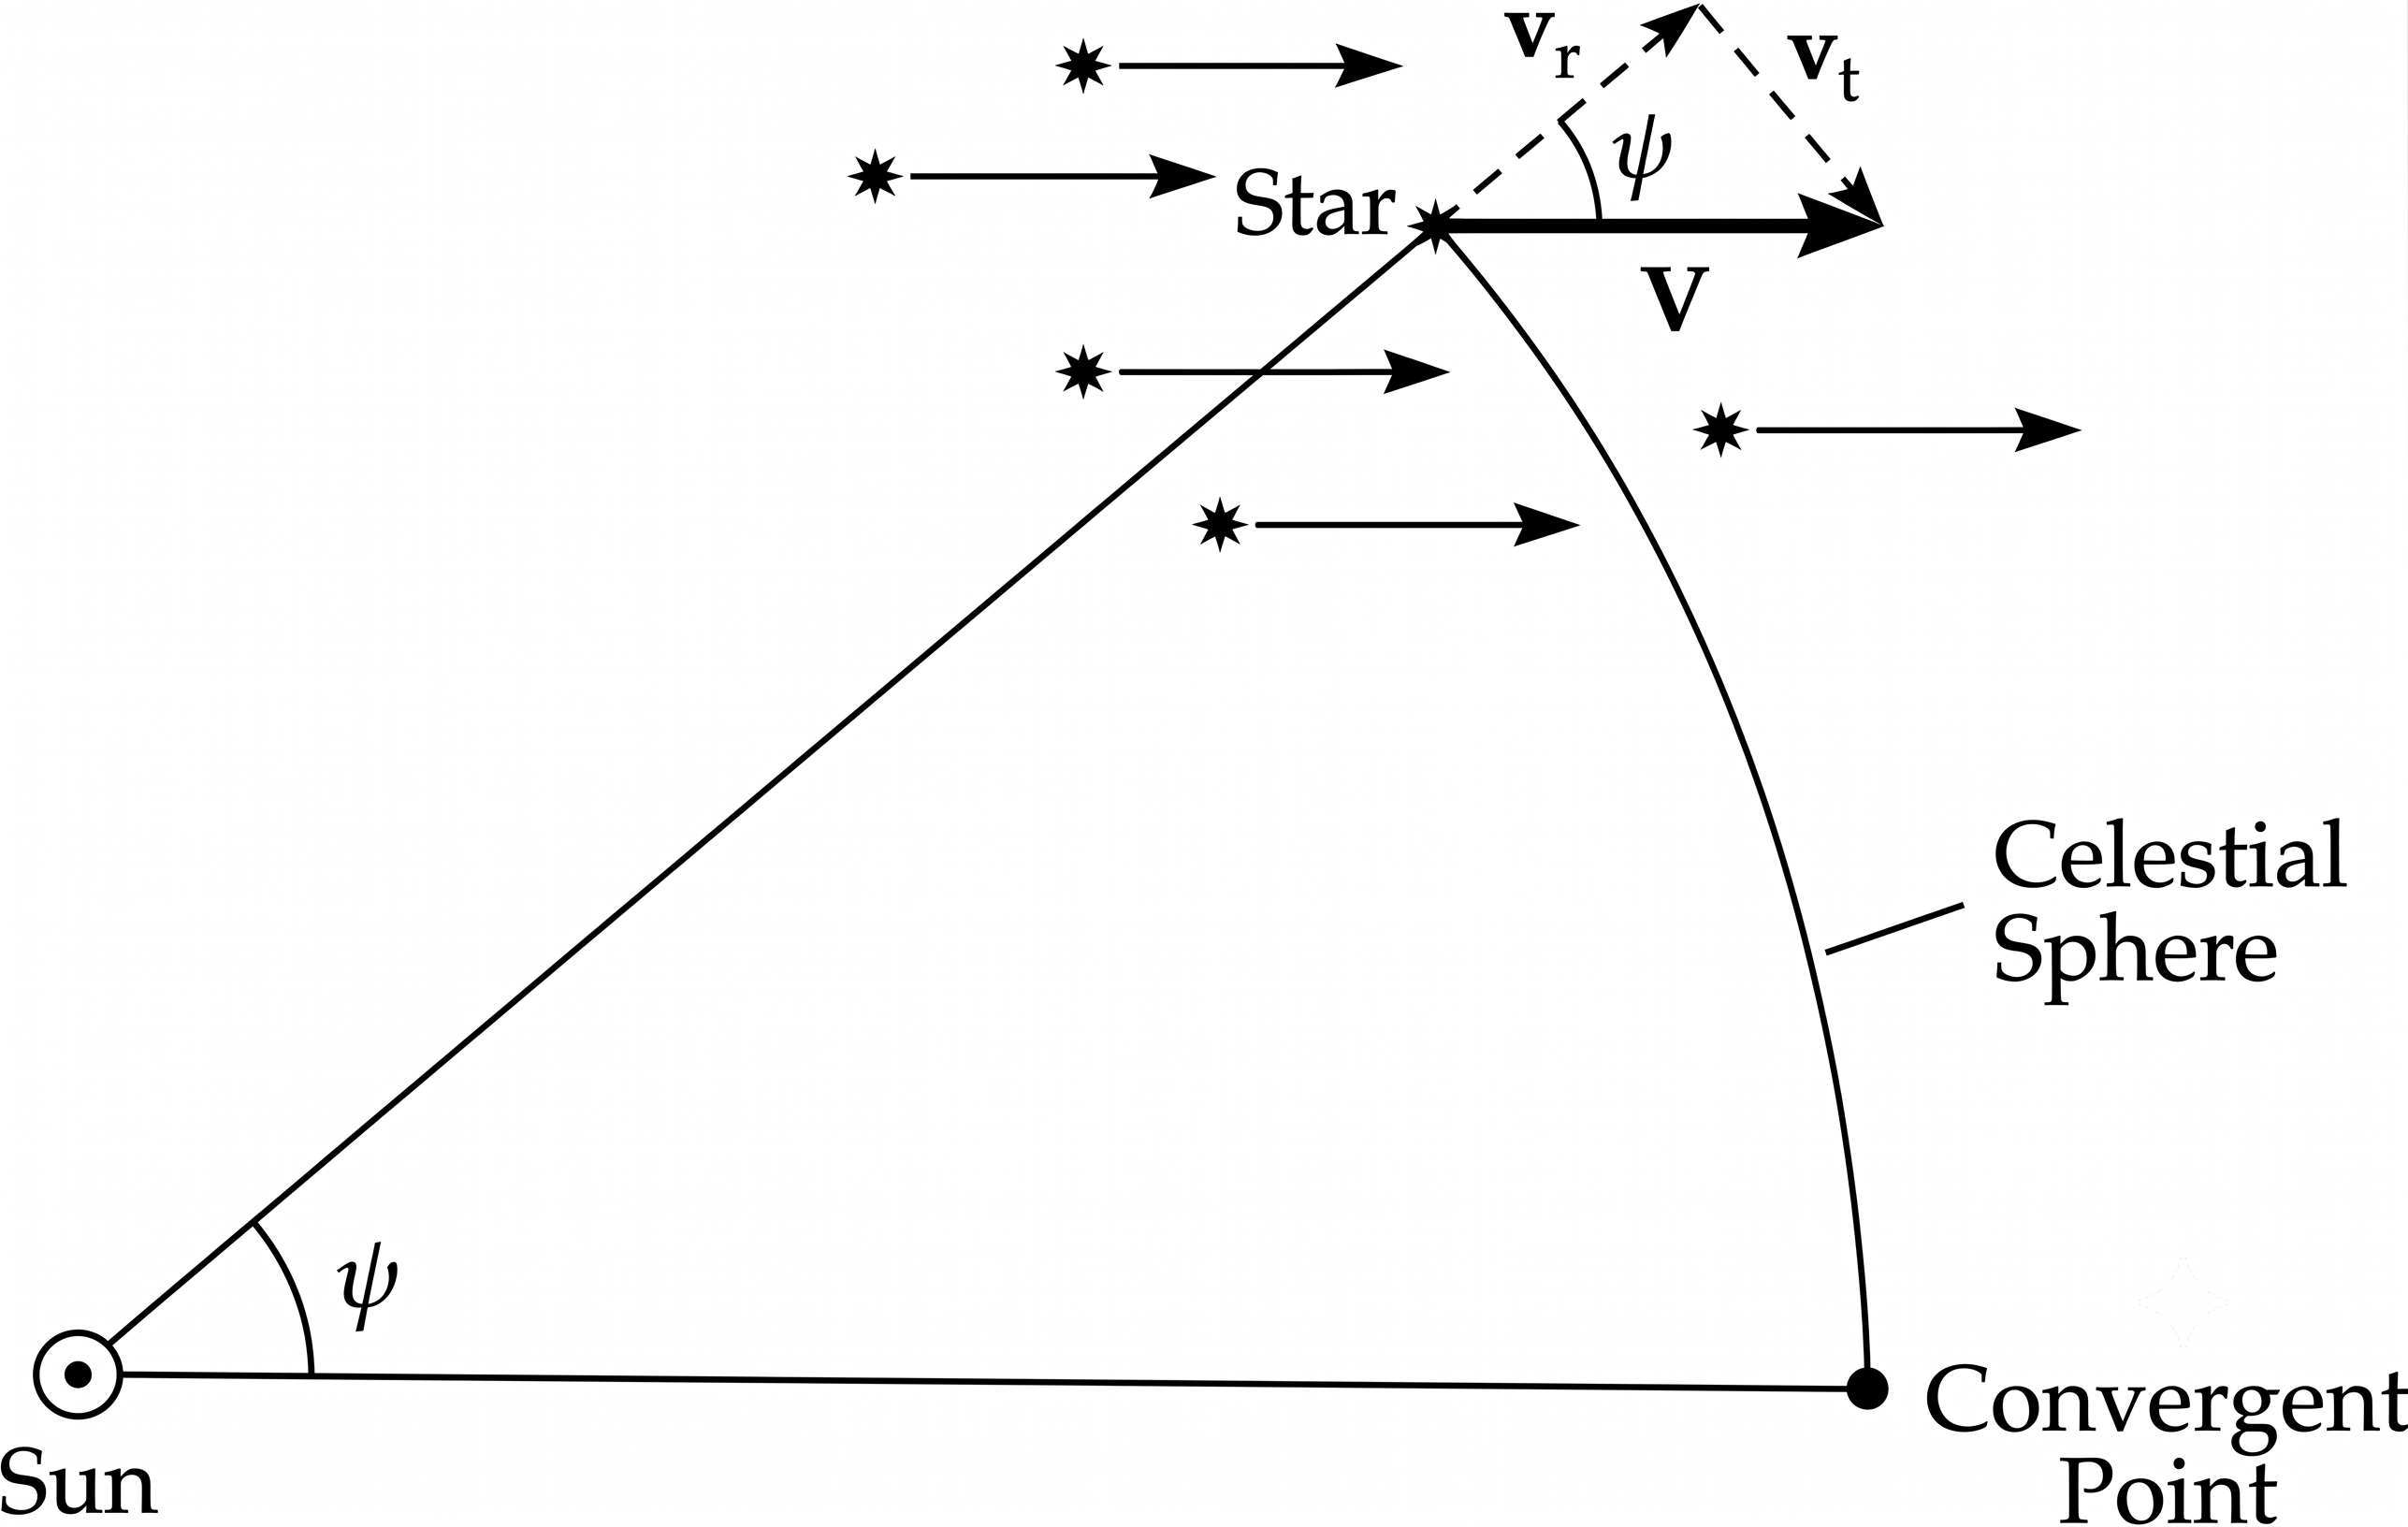
\includegraphics[width=0.95\textwidth]{assets/moving-cluster.png}
\end{minipage}

Since the total space velocity $V$ is unknown, we eliminate it using $V = V_r/\cos\psi$, then we use the relation $V_t = \mu \cdot d$ (in consistent units):
$$
V_t = V_r \tan\psi \quad \Longrightarrow \quad d = \frac{V_r \tan\psi}{\mu}
$$

\vspace{-0.3em}

The proper motion $\mu$ satisfies $\mu = V_t / d$, so the distance follows directly.

\item \textbf{Photometric and Spectroscopic Parallax}

Photometric parallax uses the apparent magnitude $m$ and an estimated absolute magnitude $M$ (inferred from the star's spectral type and luminosity class) to derive the distance modulus:
$$
m - M = 5 \log\left(\frac{D}{\mathrm{pc}}\right) - 5 + A_V
$$
If we have the spectrum of the star, we can determine $M$ (spectroscopic parallax). Taking into account the extinction $A_V \approx 3\,E(B-V)$, where $E(B-V)$ is the color excess, and measuring $(B-V)$ and $(B-V)_0$ from the spectrum, we can correct for reddening and obtain the distance.

\item \textbf{Color-Color Diagram}

When no extinction is present, there is a well-defined relation between color indices (e.g.\ $(U-B)$ and $(B-V)$) for stars of different spectral types, forming the \textbf{standard stellar locus} in the color--color diagram. In the presence of interstellar extinction, the observed colors are shifted from the intrinsic values along a \textbf{reddening vector}, with slope determined by the extinction law. The displacement along this vector in the color--color diagram gives $E(B-V)$, and hence $A_V$.

\item \textbf{Period-Luminosity Relation for Cepheids}

...
\end{enumerate}

\section{The Milky Way}

Understanding the Milky Way morphology is significantly more challenging than for external galaxies, as we are embedded within the disk and obscured by dust, making a direct global view impossible and requiring careful inference from local observations and kinematics.

\subsection{Large-Scale Structure}

The Milky Way is a typical \textbf{barred spiral galaxy} with a bright central \textbf{bulge}, a flattened \textbf{disk} containing gas, dust, and most of the young stars (Population I), and an extended \textbf{halo} populated by old stars (Population II) and globular clusters. The disk hosts the spiral structure, while the Sun lies in the disk at a galactocentric distance of about $8\,\mathrm{kpc}$. The full Galaxy spans roughly $30\text{-}50\,\mathrm{kpc}$ across, much larger than the central bulge region.

\begin{figure}[H]
    \centering
    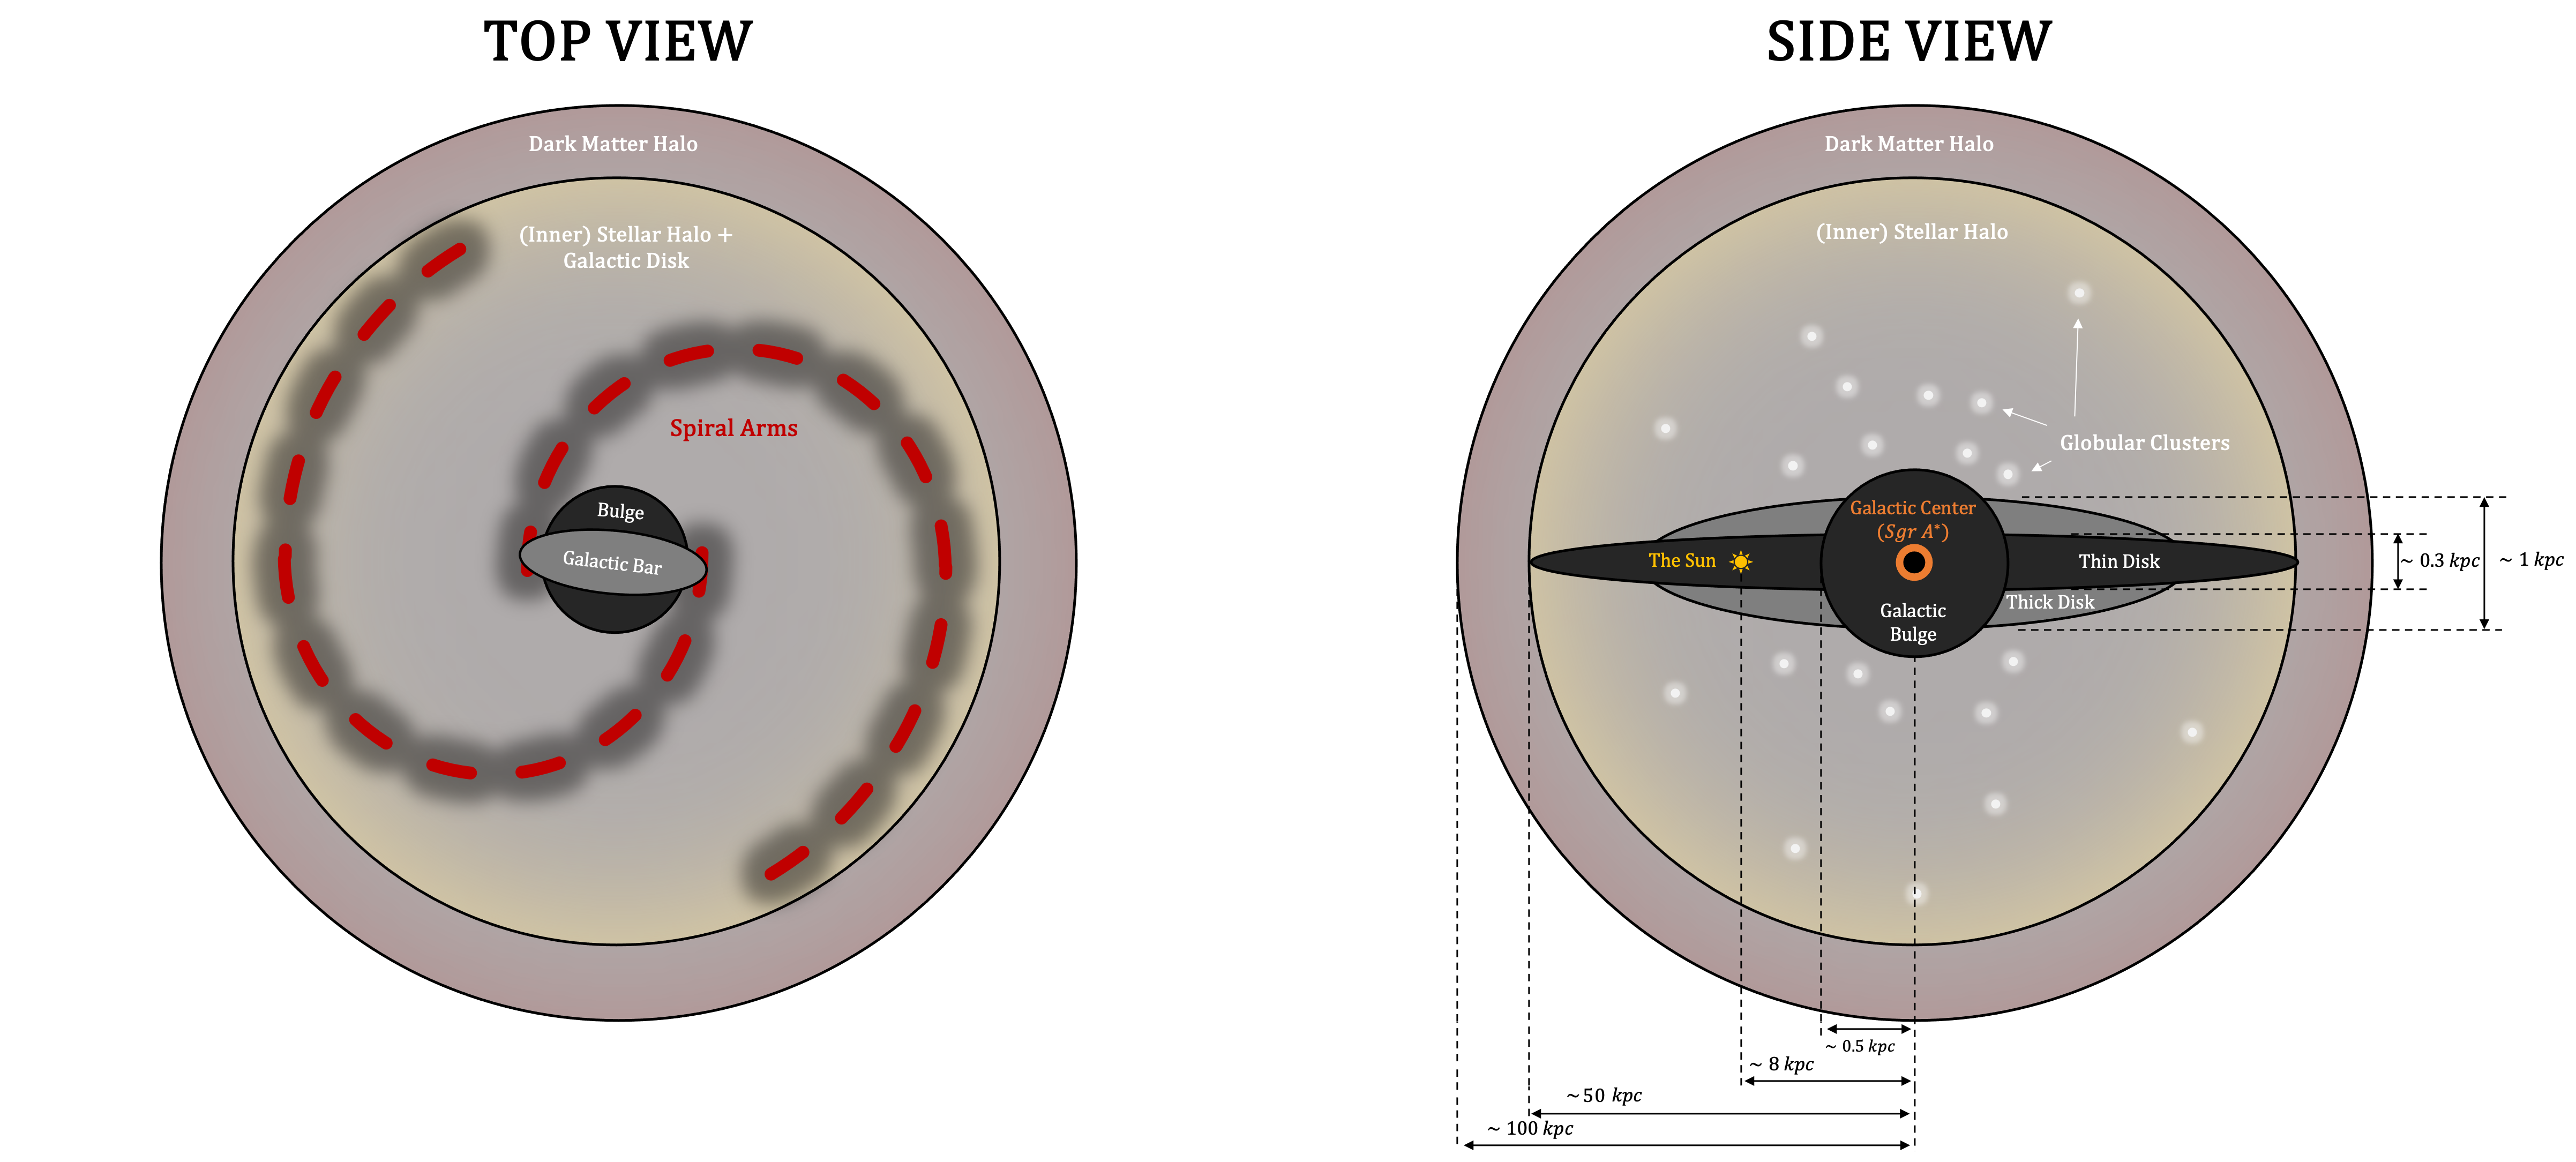
\includegraphics[width=\textwidth]{assets/mw.png}
    \captionof{figure}{Schematic top and side view of the Milky Way}
\end{figure}

\subsection{The Disk}

The disk of the Milky Way consists of a \textbf{thin disk} and a \textbf{thick disk}.

\subsubsection{Density Profile}

The stellar number density in the disk is modeled as:

$$
n(R, z) = n_0 \left( a\,e^{-|z|/h_t} + b\,e^{-|z|/h_T} \right) e^{-R/h_R}
$$

where:
\begin{itemize}[noitemsep]
    \item $n_0$ is the normalization constant (central density)
    \item $a$ and $b$ are dimensionless amplitude parameters controlling the relative contributions of the thin and thick disk components (with $a + b = 1$)
    \item $z$ is the vertical distance from the midplane of the disk, and $R$ is the radial distance from the Galactic center in the plane of the disk
    \item $h_t$, $h_T$, and $h_R$ are the \textbf{scale lengths} (or heights) of the thin disk, thick disk, and radial profile, respectively. More specifically:
    \begin{itemize}[noitemsep]
        \item $h_t$ (thin disk): $\approx 300\,\mathrm{pc}$
        \item $h_T$ (thick disk): $\approx 1\,\mathrm{kpc}$
        \item $h_R$ (radial scale length): $\approx 3.5\,\mathrm{kpc}$
    \end{itemize}
\end{itemize}
The exponential term $e^{-R/h_R}$ is nearly the same for external spiral galaxies as well.

\subsubsection{Kinematics of the Disk}

The disk exhibits a nearly flat rotation curve, a characteristic often referred to as \textbf{cold motion}:
$$
V_\odot \approx 220\,\mathrm{km/s}
$$

Stars also have random \textbf{vertical} and \textbf{radial} motions superimposed on this cold circular rotation, referred to as \textbf{hot motion}, with typical velocity dispersions of $\approx 15-25\,\mathrm{km/s}$.

There are several hypotheses for the formation of galactic disks:

\begin{itemize}
    \item One possibility is that stars form in the thin disk and then gradually acquire larger vertical velocity dispersions through repeated gravitational scattering, which thickens the disk (\textit{kinematic heating}). In this picture, more metal-rich stars tend to remain in the thin disk, while more metal-poor (Population II) stars are more often found in the thick disk. The disk also contains molecular gas (e.g.\ CO) and a diffuse interstellar medium.
    
    \item Another possibility is that the thick disk formed through the accretion or interaction of a satellite galaxy with a pre-existing thin disk. Such an encounter can heat thin-disk stars and/or deposit stars and gas at larger scale heights, producing a thicker component. In this scenario, the thick disk often rotates more slowly than the thin disk, and in some external galaxies thick components have even been observed to rotate counter to the thin disk.
\end{itemize}

\subsubsection{Mass and Luminosity of the Disk}

The total mass of the disk is approximately:

$$
M_\mathrm{disk} \approx 6 \times 10^{10}\,M_\odot\,(\text{stars}) + 0.5 \times 10^{10}\,M_\odot\,(\text{gas})
$$

and the mass-to-light ratio is:

$$
\frac{M}{L} \approx 3\,\frac{M_\odot}{L_\odot}, \quad \text{where } L_0 \approx 2 \times 10^{10}\,L_\odot
$$

\subsection{Spiral Structure}

\begin{minipage}{0.55\textwidth}
The Milky Way has a \textbf{bar} (detected by the Gaia mission, bar length $\sim 4$--$5\,\mathrm{kpc}$) and spiral arms, the most prominent being the \textbf{Sagittarius} and \textbf{Perseus} arms. The Sun lies almost midway between these two arms. The spiral structure most likely arises from \textbf{pressure (density) waves} propagating through the gas disk, triggering star formation along the arms. Spiral arms trace the distribution of $\text{H}_{II}$ regions and blue (young) stars.
\end{minipage}%
\hfill
\begin{minipage}{0.4\textwidth}
    \vspace{-1em}
    \centering
    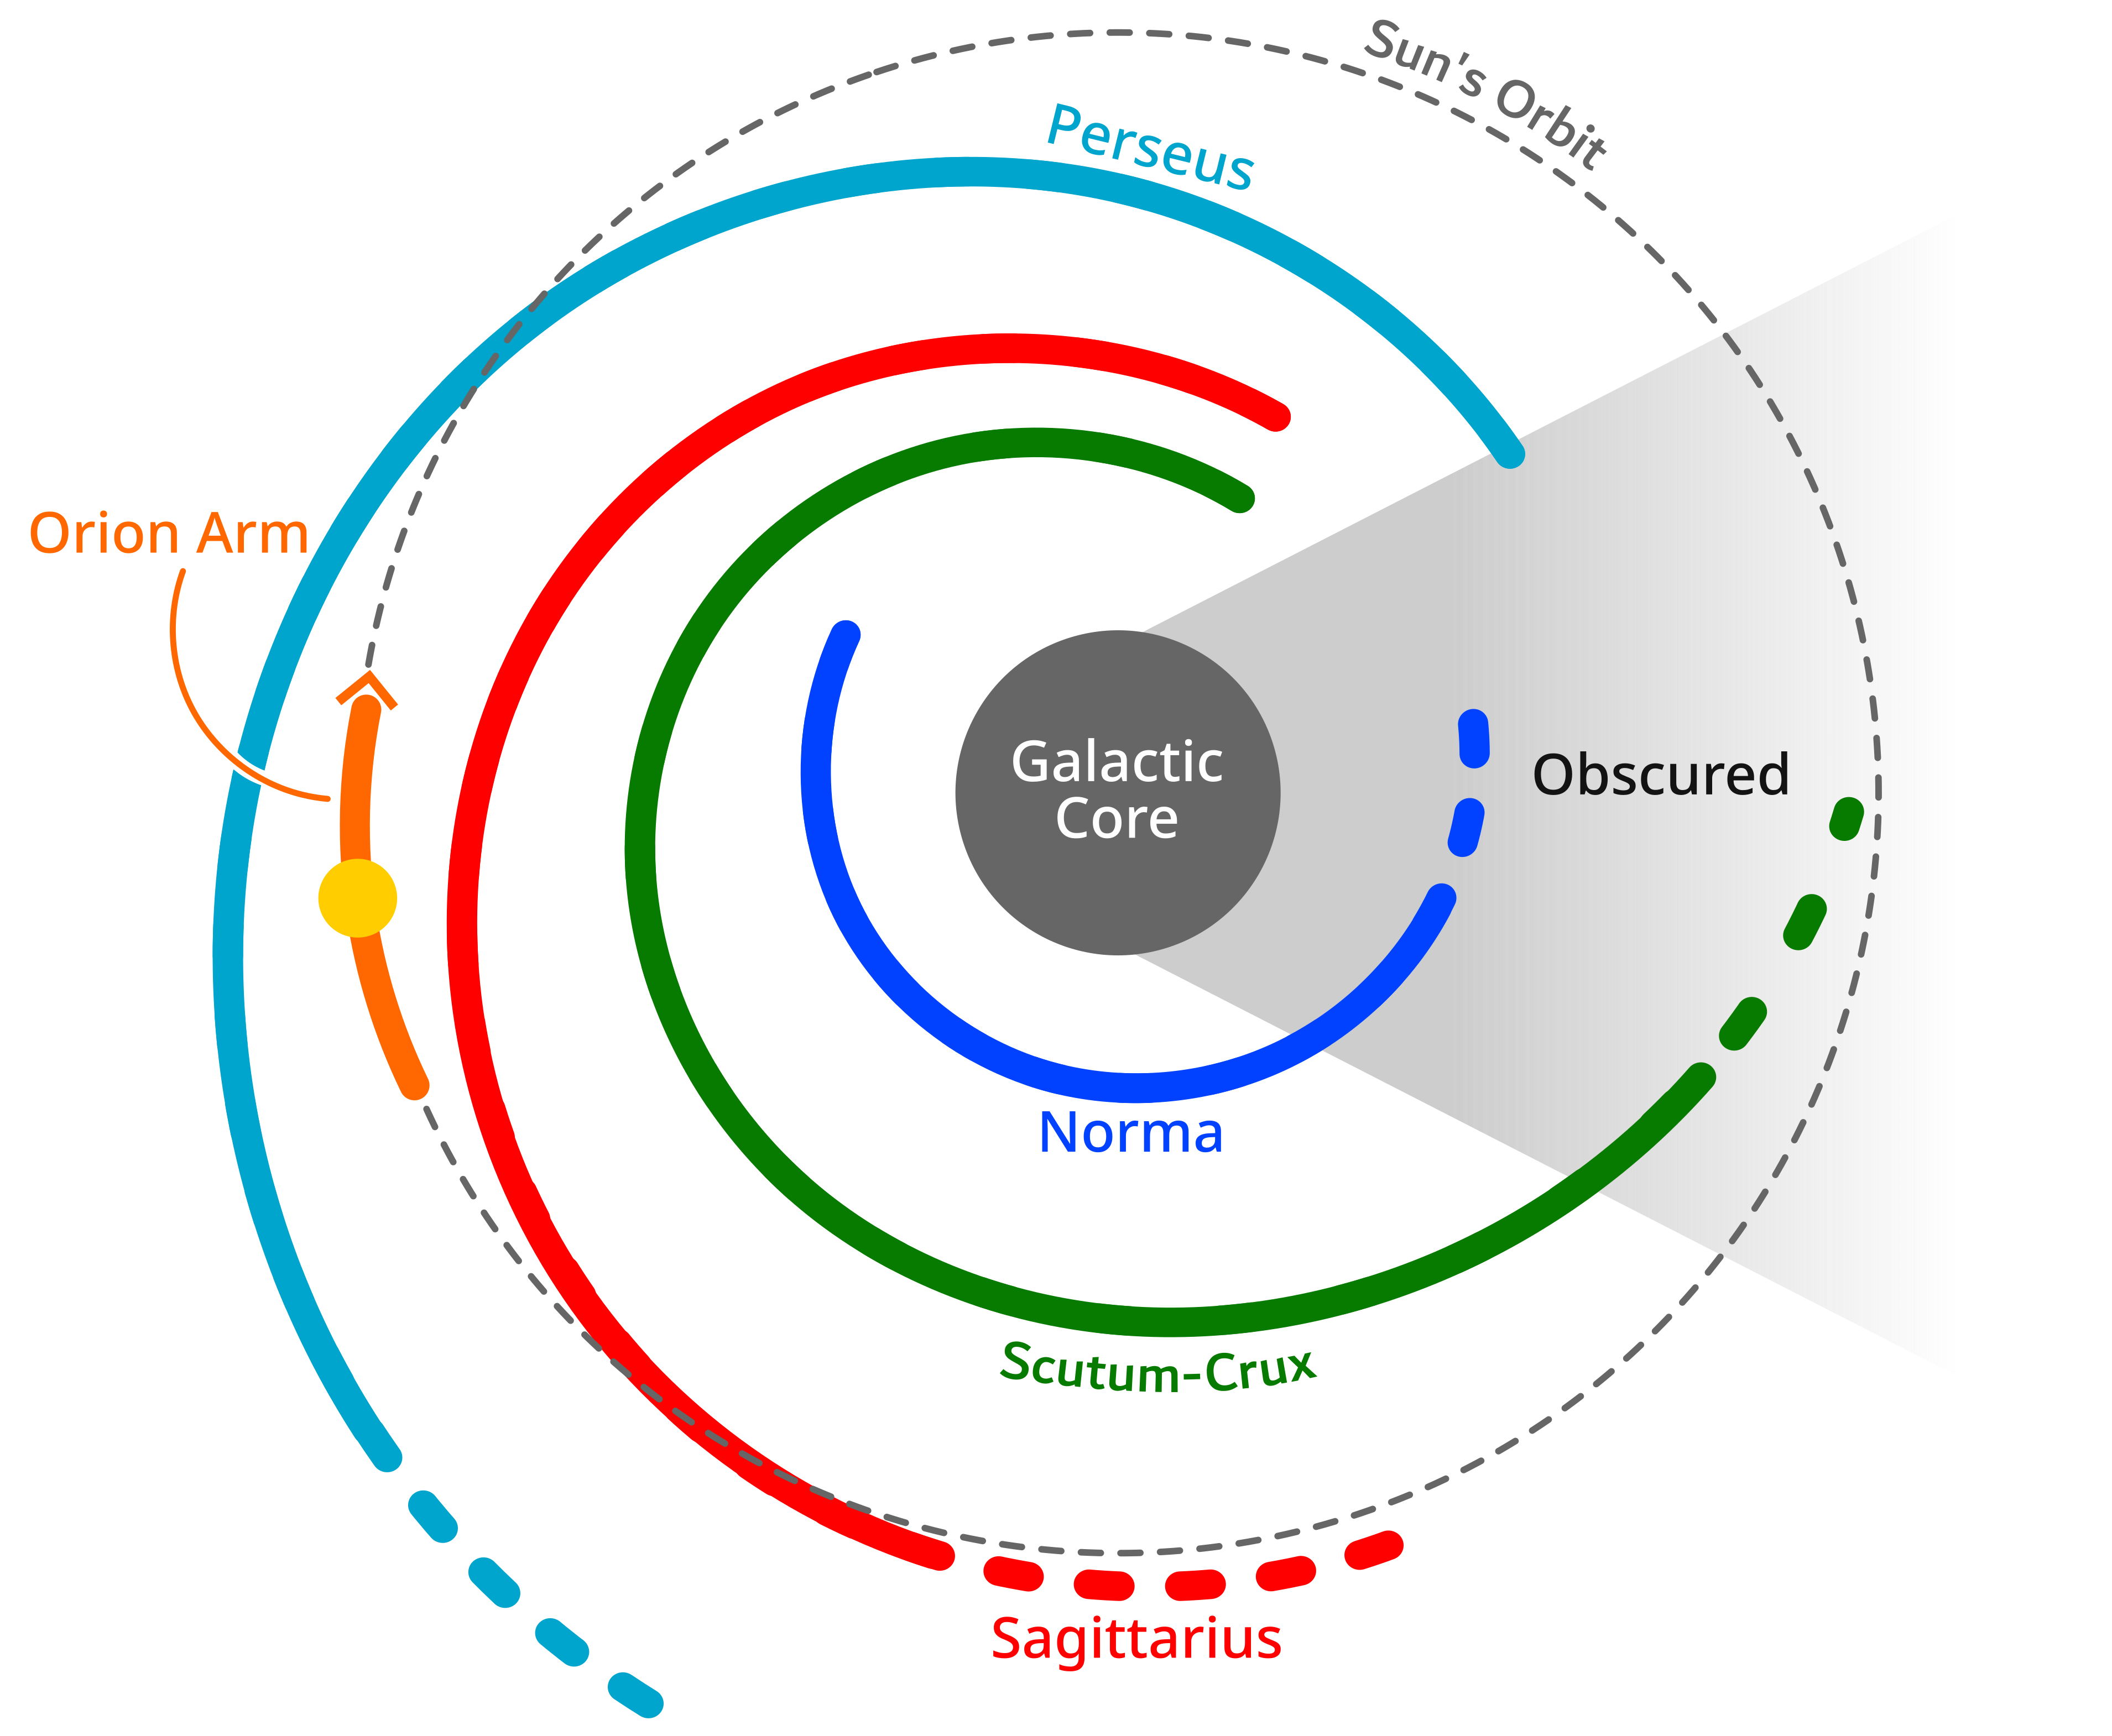
\includegraphics[width=\textwidth]{assets/spiral.png}
\end{minipage}

\subsection{The Bulge}

The \textbf{bulge} is the central, roughly spheroidal component of the Milky Way. It suffers from heavy extinction along the line of sight ($A_V \sim 28\,\mathrm{mag}$ in the optical toward the Galactic center), making it best studied in the infrared.

\subsubsection{De Vaucouleurs Profile}

If we assume spherical symmetry for the bulge, its surface brightness profile follows the \textbf{de Vaucouleurs} (or $r^{1/4}$) \textbf{law}:
$$
\log\left(\frac{I(R)}{I_e}\right) = -3.3307\left[\left(\frac{R}{R_e}\right)^{1/4} - 1\right]
$$
where $I_e = I(R_e)$, is the surface brightness ($[I] = L_\odot/pc^2$) at the \textbf{effective radius} $R_e$ ($\sim 0.7\,\mathrm{kpc}$), defined such that half the total luminosity is enclosed within $R_e$:
$$
\int_0^{R_e} I(R)\,R\,\dd{R} = \frac{1}{2}\int_0^{\infty} I(R)\,R\,\dd{R}
$$
The total surface luminosity is:
$$
L = \int_0^{\infty} I(R)\,2\pi R\,\dd{R} = 7.215\,\pi\,I_e R_e^2
$$
The de Vaucouleurs profile applies to the bulges of spiral galaxies and to elliptical galaxies.

The stellar mass in the bulge is $M_{\star,B} \approx 1.6 \times 10^{10}\,M_\odot$, with a mass-to-light ratio:
$$
\frac{M}{L} \approx 5\,\frac{M_\odot}{L_\odot}
$$

\subsection{The Halo}

The \textbf{stellar halo} is a roughly spherical, low-density component extending to $r \lesssim 35\,\mathrm{kpc}$, populated mainly by old, metal-poor \textbf{Population II} stars. It contains about 150 globular clusters distributed spherically around the Galactic center.

If we assume spherical symmetry, the stellar density in the halo falls off as:
$$
n(r) \propto r^{-\gamma}, \quad \gamma \approx 3\text{--}3.5
$$

The gaseous halo contains \textbf{high-velocity clouds} (HVCs) with $V \gtrsim 400\,\mathrm{km\,s^{-1}}$ (e.g.\ the Magellanic Stream). These gas reservoirs are thought to be the raw material from which stars form. The gaseous halo constitutes roughly $10\%$ of the total interstellar medium mass.

\subsection{The Galactic Center}

At the center of the Milky Way lies a \textbf{supermassive black hole}, \textbf{Sagittarius~A*} (Sgr~A*), which is a radio-emitting, compact source first identified as a radio source. It has a mass of $M_\bullet \approx 4 \times 10^6\,M_\odot$. Sgr~A* is also associated with \textbf{AGN} (Active Galactic Nuclei) activity, although it is currently in a quiescent state.
From cosmic ray and dust particle studies, we know that the Milky Way harbors a large-scale \textbf{magnetic field} of roughly $B \approx 4\,\mu\mathrm{G}$.

\section{Stellar Statistics: The Population of Stars}

The observed distribution of stars in apparent magnitude is related to their intrinsic luminosity function and spatial distribution. The same principles apply to galaxies as well, where we relate the observed galaxy counts to the galaxy luminosity function and spatial distribution.

\subsection{The Luminosity Function}

\begin{minipage}{0.62\textwidth}
    The \textbf{luminosity function} $\Phi(M)$ describes the number density of stars (or galaxies) per unit absolute magnitude $M$ per unit volume. 
    Consider a small number of stars $\dd{N}$ in a range of magnitudes $[M, M + \dd{M}]$ and positions in a volume element $\dd^3\vec{x}$ around $\vec{x}$:
    $$
    \dd{N} \equiv \Phi(M,\vec{x})\,\dd{M}\,\dd^3\vec{x}
    $$
    Assuming the magnitude is \textit{independent} of position, we can separate the luminosity function from the spatial distribution:
    $$
    \dd{N} = \Phi(M)\,\dd{M}\cdot\nu(\vec{x})\,\dd^3\vec{x}
    $$
    where $\nu(\vec{x})$ is the \textbf{numerical density}.
\end{minipage}%
\hfill
\begin{minipage}{0.36\textwidth}
    \centering
    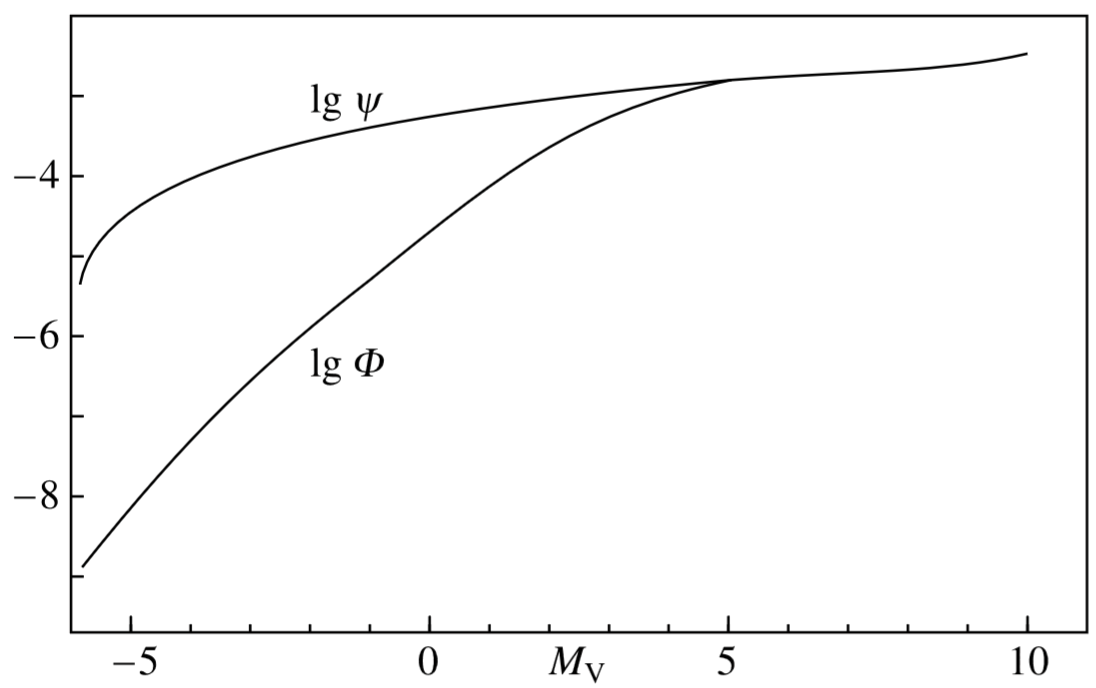
\includegraphics[width=\textwidth]{assets/luminosity-function.png}
    \captionof{figure}{Luminosity function $\Phi$ and the initial luminosity function $\Psi$ for main sequence stars in the solar neighbourhood \cite{karttunen}.}
\end{minipage}

\vspace{-0.5em}

\subsection{The Fundamental Equation of Stellar Statistics}

We want to relate the observable \textbf{star counts} $A(m)$, which is the number of stars per unit solid angle brighter than apparent magnitude $m$, to the luminosity function and the spatial distribution.

Consider a spherical shell at distance $s$ (in pc) with thickness $\dd{s}$ and solid angle $\omega$.

\medskip

\begin{minipage}{0.58\textwidth}
The number of stars in the absolute magnitude range $[M, M+\dd{M}]$ in this shell is:
$$
\dd{N} = \Phi(M)\,\dd{M}\cdot\nu(\vec{x})\,\dd^3\vec{x} = \Phi(M)\,\dd{M}\dd{n}
$$
and the total differential star counts:
$$
\frac{\dd^2 N}{\dd{m}\,\dd{M}} = \Phi(M)\left.\dfrac{\dd{n}}{\dd{m}}\right|_M
$$
\end{minipage}%
\hfill
\begin{minipage}{0.4\textwidth}
    \centering
    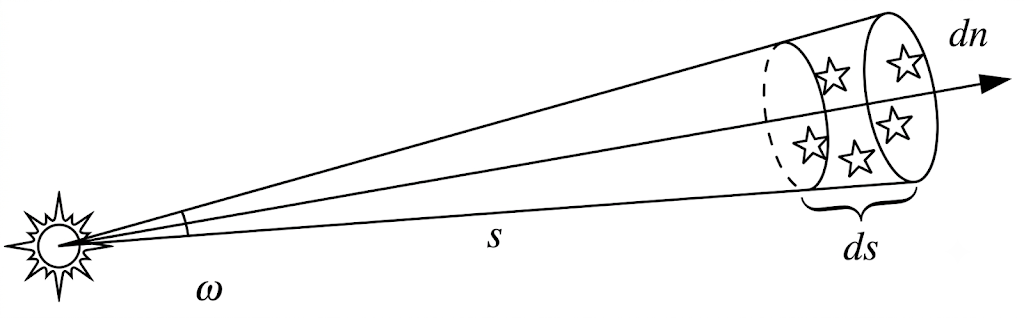
\includegraphics[width=\textwidth]{assets/star-counts.png}
    \captionof{figure}{A spherical shell at distance $s$ with thickness $\dd{s}$ and solid angle $\omega$.}
\end{minipage}

\medskip

Using the relation $m - M = 5\log s - 5$ (ignoring extinction for simplicity), we have:

$$
\frac{\dd^2 N}{\dd{m}\,\dd{M}} = \Phi(M)\dfrac{\dd{n}}{\dd{s}}\left(\dfrac{\partial s}{\partial m}\right)_M
$$

Since the number of stars in the shell element is $\dd{n} = \omega\,s^2\,\dd{s}\,\nu(s)$, we get $\frac{\dd{n}}{\dd{s}} = \omega\,s^2\,\nu(s)$.
The \textbf{star counts} therefore become:
$$
A(m) \equiv \frac{\dd{N}}{\dd{m}} = \int_{-\infty}^{+\infty} \frac{\dd^2 N}{\dd{m}\,\dd{M}}\,\dd{M} = \omega\int_{-\infty}^{+\infty} \Phi(M)\left(\frac{\partial s}{\partial m}\right)_M s^2\,\nu(s)\,\dd{M}
$$

We can express this integral in terms of the distance $s$ instead of $M$. From the distance modulus ($m - M = 5 \log s - 5$), we observe that at a fixed apparent magnitude $m$:
\begin{itemize}[noitemsep]
    \item When $M \to -\infty$ (extremely bright stars), we can see them at $s \to +\infty$.
    \item When $M \to +\infty$ (extremely faint stars), we can see them only at $s \to 0$.
\end{itemize}

Moreover, differentiating the distance modulus, we find that:
$$
\left(\frac{\partial M}{\partial s}\right)_m = -\left(\frac{\partial m}{\partial s}\right)_M \quad \Longrightarrow \quad \dd{M} = -\left(\frac{\partial m}{\partial s}\right)_M \dd{s}
$$
Substituting this into the integral and taking into account the integration limits, we get:
$$
\left(\frac{\partial s}{\partial m}\right)_M \dd{M} = -\left(\frac{\partial s}{\partial m}\right)_M \left(\frac{\partial m}{\partial s}\right)_M \dd{s} = -\dd{s}
$$

Evaluating the integral from $s = +\infty$ to $s = 0$ with the minus sign inverts the bounds, yielding the \textbf{Fundamental Equation of Stellar Statistics}:

$$
\boxed{
    A(m) = \omega \int_0^{\infty} \Phi(M)\,s^2\,\nu(s)\,\dd{s}
}
$$

where the absolute magnitude $M = m - 5\log s + 5$ links $m$, $s$, and $M$ at each point along the LOS.

\subsection{The Malmquist Bias}

Observational surveys are typically \textbf{magnitude-limited}, meaning that they detect only stars or galaxies brighter than a limiting apparent magnitude $m_\mathrm{lim}$. This introduces the \textbf{Malmquist bias}: at larger distances, only the intrinsically brighter, and often more massive, objects are included, biasing the inferred properties.
The observed distribution is therefore skewed toward intrinsically bright sources at large distances. As a result, the mean absolute magnitude of the sample is systematically \textit{brighter} than the true mean of the population: $\langle M_\mathrm{obs} \rangle < \langle M_\mathrm{true} \rangle$.

\vspace{-0.3em}

\begin{figure}[H]
    \centering
    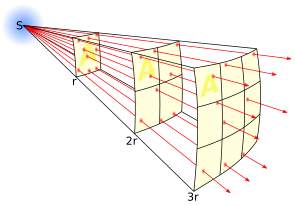
\includegraphics[height=0.2\textheight]{assets/inverse-square-law.png}
    \hspace{3em}
    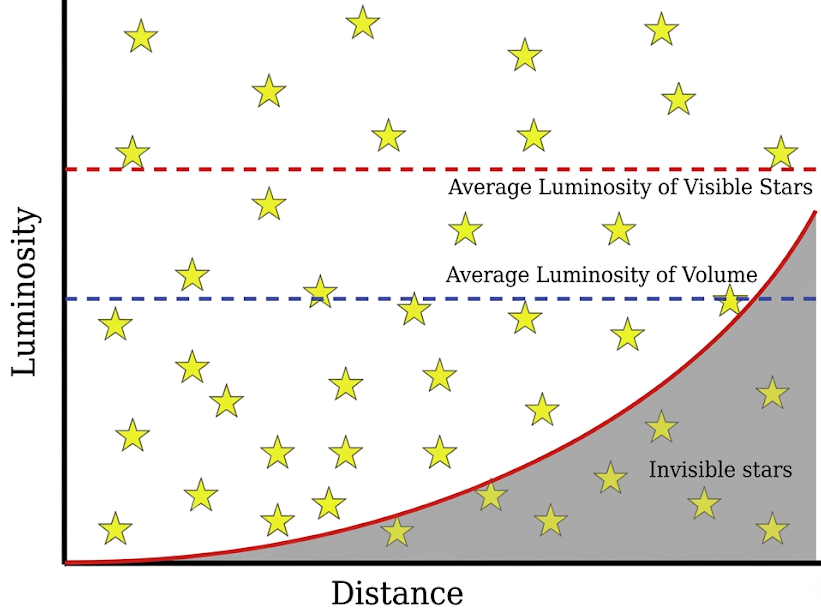
\includegraphics[height=0.2\textheight]{assets/malmquist.png}
    \vspace{-0.3em}
\captionof{figure}{Malmquist bias. Left: the inverse-square law causes flux to decrease with distance \cite{malmquist_img}. Right: a magnitude-limited survey preferentially detects intrinsically brighter stars.}
\end{figure}

\vspace{-0.3em}

One can convert a magnitude-limited sample to a \textbf{volume-limited} sample by restricting to the distance at which even the faintest objects of interest would still be detected.

\textbf{Proof:}

Let $A(m)$ be the total number of stars observed with apparent magnitude $m$. The mean absolute magnitude of a sample of stars with apparent magnitude $m$ is given by the ratio of integrals over the magnitude and distance $s$:
$$
\langle M \rangle_m = \frac{\int_{-\infty}^{+\infty} dM \, M \, \frac{d^2 N}{dm\,dM}}{\int_{-\infty}^{+\infty} dM \, \frac{d^2 N}{dm\,dM}} = \frac{\omega \int_0^\infty ds \, M \, \varphi(M) \, s^2 \nu(s)}{\omega \int_0^\infty ds \, \varphi(M) \, s^2 \nu(s)}
$$
We know that the derivative of $A(m)$ with respect to $m$ is:
$$
\frac{dA}{dm} = \omega \int_0^\infty ds \, \frac{d\varphi}{dm} \, s^2 \nu(s)
$$
Since apparent and absolute magnitudes differ only by the distance modulus (which is independent of $m$ and $M$ locally), we have $dm = dM$, which implies $\frac{d\varphi}{dm} = \frac{d\varphi}{dM} \frac{dM}{dm} = \frac{d\varphi}{dM}$. Therefore:
$$
\frac{dA}{dm} = \omega \int_0^\infty ds \, \frac{d\varphi}{dM} \, s^2 \nu(s)
$$
We can write the expected value of $\frac{1}{\varphi}\frac{d\varphi}{dM}$ at a given $m$ as:
$$
\left\langle \frac{1}{\varphi} \frac{d\varphi}{dM} \right\rangle_{\!m} = \frac{\omega \int_0^\infty ds \left[ \frac{1}{\varphi} \frac{d\varphi}{dM} \right] \varphi(M) \, s^2 \nu(s)}{\omega \int_0^\infty ds \, \varphi(M) \, s^2 \nu(s)} = \frac{1}{A(m)} \frac{dA}{dm}
$$
\textit{(With a similar computation, one can also show that $\left\langle \frac{1}{\varphi} \frac{d^2\varphi}{dM^2} \right\rangle_m = \frac{1}{A} \frac{d^2 A}{dm^2}$).}

Assuming that the luminosity function $\varphi(M)$ is a Gaussian (which is at least true for a specific stellar class), with true mean $M_0$ and variance $\sigma^2$:
$$
\varphi(M) = \frac{1}{\sqrt{2\pi\sigma^2}} e^{-\frac{(M-M_0)^2}{2\sigma^2}} \quad \Longrightarrow \quad \frac{d\varphi}{dM} = \varphi(M) \frac{M_0 - M}{\sigma^2}
$$
Substituting this derivative into our expected value equation:
$$
\left\langle \frac{1}{\varphi} \frac{d\varphi}{dM} \right\rangle_{\!m} = \frac{\omega \int_0^\infty ds \, \varphi(M) \left( \frac{M_0 - M}{\sigma^2} \right) s^2 \nu(s)}{\omega \int_0^\infty ds \, \varphi(M) \, s^2 \nu(s)} = \left\langle \frac{M_0 - M}{\sigma^2} \right\rangle_{\!m} = \frac{M_0 - \langle M \rangle_m}{\sigma^2}
$$
Equating this to $\frac{1}{A}\frac{dA}{dm}$, we get:
$$
\frac{M_0 - \langle M \rangle_m}{\sigma^2} = \frac{1}{A} \frac{dA}{dm}
\qquad\Rightarrow\qquad
\langle M \rangle_m = M_0 - \sigma^2 \underbrace{\left( \frac{1}{A} \frac{dA}{dm} \right)}_{> 0}
$$
Since the number of observed stars $A(m)$ naturally increases as we look at fainter apparent limits (higher $m$), the derivative $\frac{dA}{dm}$ is strictly positive. Therefore, we rigorously obtain:
$$
\langle M \rangle_m < M_0
$$
which formally proves the Malmquist bias: the observed mean absolute magnitude $\langle M \rangle_m$ is systematically brighter (numerically smaller) than the true population mean $M_0$.

\textit{Moreover, for the variance: $\langle \sigma^2 \rangle_m = \sigma^2 + \sigma^4 \frac{d^2 \ln A}{dm^2}$. If this derivative is 0, the density is constant (uniform distribution).}

\section{Kinematics of the Milky Way}

Milky way does not behave as a rigid body, but rather exhibits \textbf{differential rotation}, where the orbital velocity of stars depends on their distance from the Galactic center.

Let us suppose the stars are moving in circular orbits about the galactic centre (\cref{fig:mw-kinematics}). This approximation is acceptable for population I stars and gas. The star $S$, seen from the Sun $\odot$ at galactic longitude $l$ at distance $r$, has circular velocity $V$ at a distance $R$ from the centre. 

\begin{figure}[H]
    \centering
    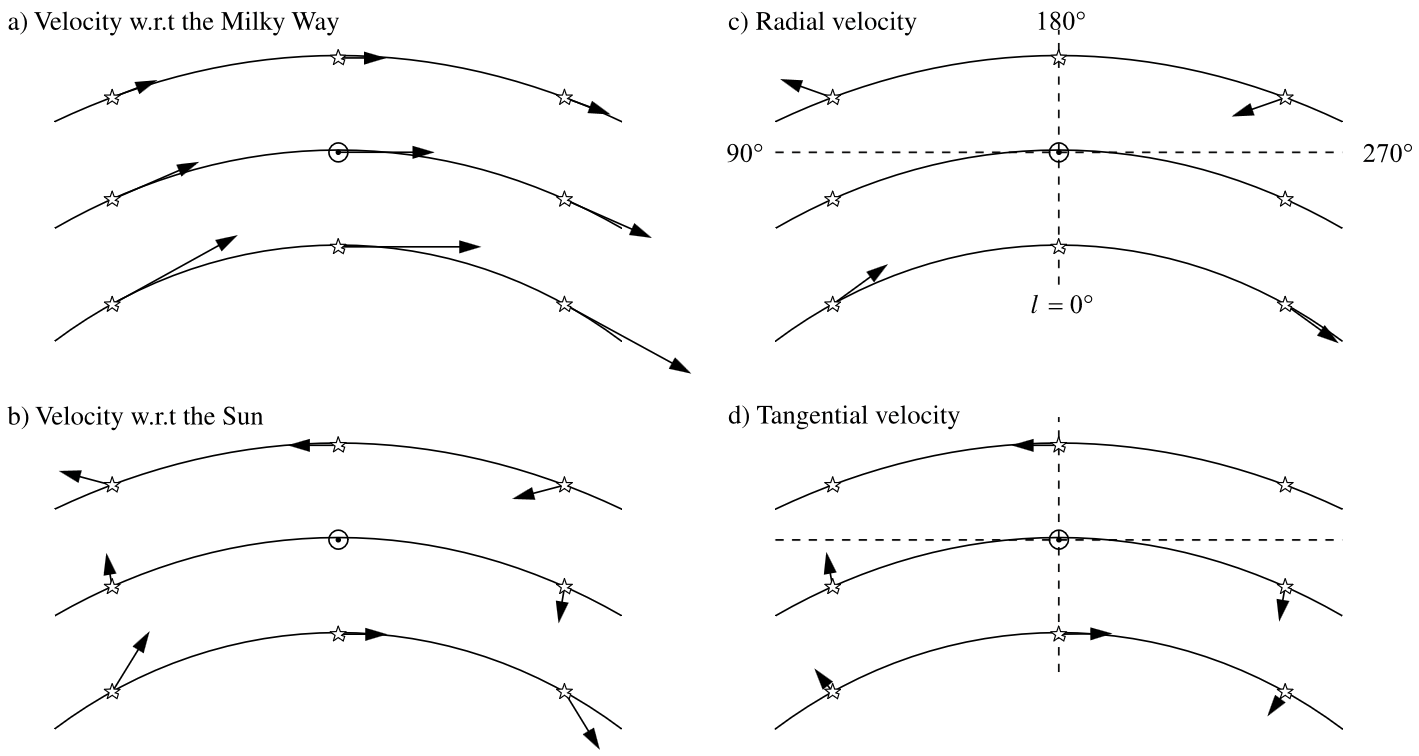
\includegraphics[width=0.95\textwidth]{assets/mw-kinematics.png}
    \captionof{figure}{The effect of differential rotation on the radial velocities and proper motions of stars \cite{karttunen}. \textbf{(a)} Near the Sun the orbital velocities of stars decrease outwards in the Galaxy. \textbf{(b)} The relative velocity with respect to the Sun is obtained by subtracting the solar velocity from the velocity vectors in (a). \textbf{(c)} The radial components of the velocities with respect to the Sun. This component vanishes for stars on the same orbit as the Sun. \textbf{(d)} The tangential components of the velocities.}
    \label{fig:mw-kinematics}
\end{figure}

\subsection{Oort's Constants}

We want to study the velocity of stars in a neighborhood of the Sun.

\vspace{-0.5em}

\begin{figure}[H]
\begin{minipage}{0.4\textwidth}
    \centering
    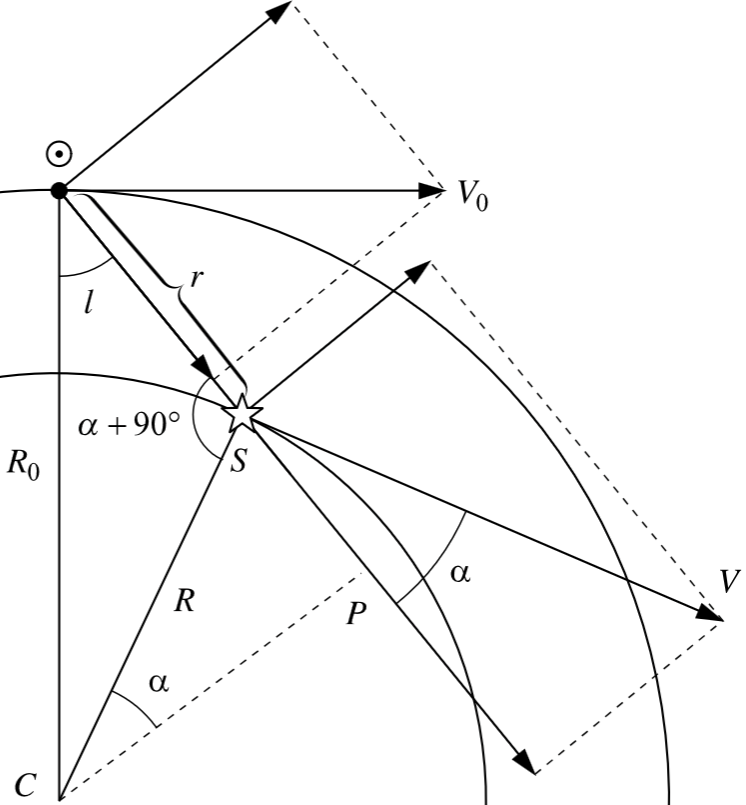
\includegraphics[width=0.98\textwidth]{assets/oort.png}
\end{minipage}%
\hfill
\begin{minipage}{0.55\textwidth}
    \captionof{figure}{In order to derive Oort's formulas, the velocity vectors of the Sun and the star S are divided into components along the line $\odot S$ and normal to it \cite{karttunen}.}
    \begin{itemize}
        \item $r$ is the distance between the Sun and the star of interest.
        \item $R$ is the distance of the star from the Galactic center.
        \item $R_0$ is the distance of the Sun from the Galactic center.
        \item $V$ is the circular velocity of the star at distance $R$.
        \item $V_0$ is the circular velocity of the Sun.
        \item $l$ is the galactic longitude of the star.
        \item $\alpha$ is the angle used to project the velocity components in the geometry.
    \end{itemize}
\end{minipage}
\end{figure}

We have $r \ll R$ and $R \approx R_0$. The relative radial velocity $v_r$ of the star with respect to the Sun is given by:
$$
v_r = V \cos \alpha - V_0 \sin l = \omega R \cos \alpha - \omega_0 R_0 \sin l
$$
The triangle $\odot C P$ gives us the relation $R \sin \alpha = R_0 \cos l - r$. Substituting this into the expression:
$$
v_t = R_0(\omega - \omega_0) \cos l - \omega r
$$
Oort noted that in the close neighbourhood of the Sun ($r \ll R_0$), the difference of the angular velocities will be very small. Therefore we can approximate it by keeping only the first term of the Taylor series in the neighbourhood of $R = R_0$:
$$
\omega - \omega_0 = \left(\frac{d\omega}{dR}\right)_{R=R_0} (R - R_0) + \ldots
\qquad \Rightarrow \qquad
\omega-\omega_0\approx\frac{1}{R_0^2}\left[R_0\left(\frac{dV}{dR}\right)_{R=R_0}-V_0\right](R-R_0)
$$
Where we used $\omega=V/R$ and $V(R_0)=V_0$ to obtain the right equation. For $R\approx R_0\gg r$, the difference $R-R_0\approx -r\cos l$ ($\cos l \approx 1$). We can thus approximate the \textbf{radial relative velocity}:
$$
v_r\approx\left[\frac{V_0}{R_0}-\left(\frac{dV}{dR}\right)_{R=R_0}\right]r\cos l\sin l
$$
applying $2\sin\alpha\cos\alpha = \sin2\alpha$ and aggregating the constants, we can write it as:
$$
v_r\approx A r\sin 2l
$$
where $A$ is a characteristic parameter of the solar neighbourhood, the \textbf{first Oort constant}:
$$
A=\tfrac{1}{2}\left[\frac{V_0}{R_0}-\left(\frac{dV}{dR}\right)_{R=R_0}\right]
$$
For the \textbf{tangential relative velocity}, one similarly obtains, since $\omega r\approx\omega_0 r = V_0/R_0\; r$:
$$
v_t\approx\left[\frac{V_0}{R_0}-\left(\frac{dV}{dR}\right)_{R=R_0}\right]r\cos^2 l-\dfrac{V_0}{R_0} r
$$
applying $2\cos^2 l=1+\cos 2l$, substituting $A$ and aggregating the other constants, we get:
$$
v_t\approx A r\cos 2l + B r
$$
The proper motion is given by $\mu = v_t / r$:
$$
\mu \approx A \cos 2l + B
$$
with $B$ being the \textbf{second Oort constant}:
$$
B=-\tfrac{1}{2}\left[\frac{V_0}{R_0}+\left(\frac{dV}{dR}\right)_{R=R_0}\right]
$$

For the Sun's neighbourhood, the Oort constants are measured to be:

\begin{minipage}[t]{0.52\textwidth}
    $$
    A = 14.8 \pm 0.8 \; \frac{\text{km/s}}{\text{kpc}}, \quad B = -12.4 \pm 0.6 \; \frac{\text{km/s}}{\text{kpc}}
    $$

    \vfill

    \captionof{figure}{The velocity components due to differential rotation according to Oort's formulas as functions of galactic longitude \cite{karttunen}. \textbf{(a)} Radial velocities for objects at a distance of 1 and 2 kpc. The longitude at which the radial velocity vanishes depends on the distance; Oort's formulas are valid only in the close vicinity of the Sun. \textbf{(b)} Proper motions: the amplitude of the curve is A, its mean value is B}
\end{minipage}%
% \hfill
\begin{minipage}[t]{0.45\textwidth}
    \centering
    \vspace{-0.5em}
    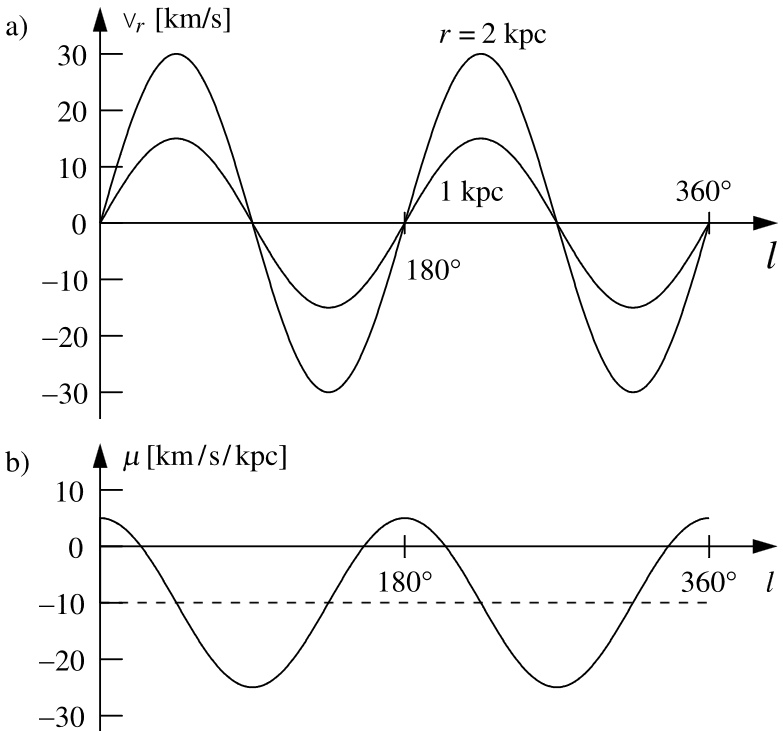
\includegraphics[width=\linewidth]{assets/oort-2.png}
\end{minipage}

The Oort constants satisfy some remarkably elegant relations. First, subtracting $B$ from $A$ yields the angular velocity of the Local Standard of Rest (LSR) around the Galactic centre:
$$
A - B = \omega_0 \approx 0.0053'' \text{ yr}^{-1}
$$
Conversely, adding the two constants provides the gradient of the circular velocity curve at the Sun's galactocentric distance ($R_0$):
$$
A + B = -\left(\frac{dV}{dR}\right)_{R=R_0} \approx -5 \text{ km s}^{-1}
$$

By observing extragalactic objects as stationary reference points, the circular velocity of the LSR can be independently determined as $V_0 \approx 220 \text{ km s}^{-1}$. Combining this value with the angular velocity $\omega_0$ allows for a direct estimate of our distance to the Galactic centre, positioning $R_0$ at approximately $8.5 \text{ kpc}$.
Consequently, the Sun's orbital period around the Galaxy can be calculated to be roughly $2.5 \times 10^8$ years. Given the solar age of nearly $5 \times 10^9$ years, it follows that the Sun has completed approximately 20 full revolutions around the Galactic centre since its formation.



\subsubsection{The Distribution of Interstellar Matter (Tangential Point Method)}

Radio radiation from interstellar gas, in particular the 21\,cm line of \textbf{neutral hydrogen} ($\text{H}_\text{I}$), is not significantly absorbed or scattered by interstellar dust, unlike optical light. 

\begin{minipage}{0.57\textwidth}
    This makes radio observations an exceptionally powerful tool for mapping the large-scale structure of the Milky Way, allowing us to detect signals even from clouds on the far side of the Galaxy.
    However, the position of a radio source along the line of sight cannot be read off directly: we can measure the \textit{direction} of a cloud on the sky, but not its distance. An indirect method based on the \textbf{differential rotation} of the Galaxy provides the solution.

    Consider a set of $\text{H}_\text{I}$ clouds $P_1, P_2, \ldots$ lying along a line of sight at Galactic longitude $l$ (with $-90^\circ < l < 90^\circ$). Each cloud moves on a roughly circular orbit around the Galactic center. Since the angular velocity $\omega(R)$ increases inward (differential rotation), different clouds along the same line of sight will have different radial velocities with respect to the Sun.
\end{minipage}%
\hfill
\begin{minipage}{0.4\textwidth}
    \centering
    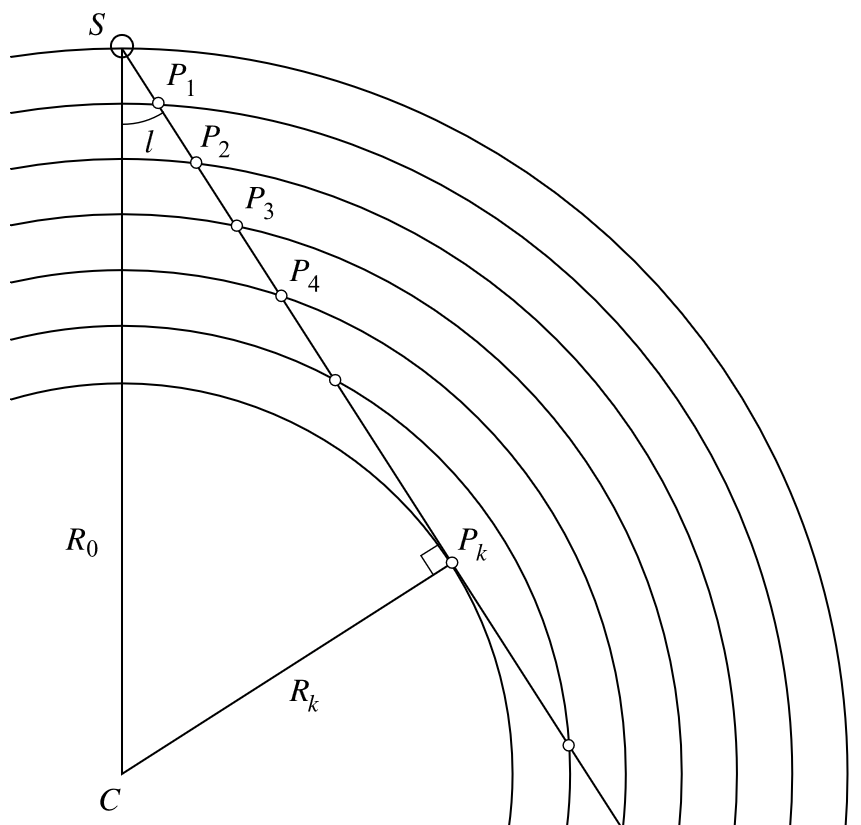
\includegraphics[width=\textwidth]{assets/HI-dist.png}
    \captionof{figure}{Clouds $P_1, P_2, \ldots$ seen in the same direction $l$ at various distances along the LOS \cite{karttunen}.}
\end{minipage}

\begin{minipage}{0.5\textwidth}
    \centering
    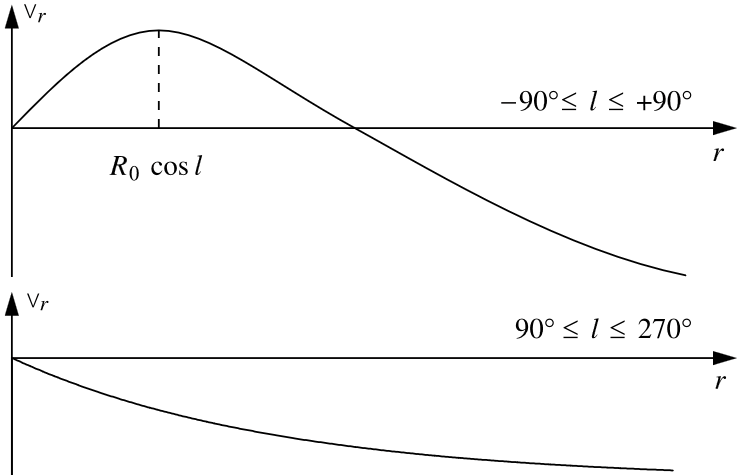
\includegraphics[width=0.9\textwidth]{assets/v_r.png}
    \captionof{figure}{The observed radial velocity as a function of distance $r$ along the line of sight \cite{karttunen}.}
\end{minipage}%
\hfill
\begin{minipage}{0.45\textwidth}
The radial velocity of a cloud at Galactocentric distance $R$ along the line of sight $l$ is $v_r = R(\omega(R) - \omega_0)\sin l$. As we move along the line of sight, $v_r$ increases until we reach the \textbf{tangent point} $P_k$, where the line of sight is tangent to the circular orbit at $R_k = R_0 \sin l$. At this point the radial velocity reaches its maximum $v_{r,\mathrm{max}} = R_k\bigl(\omega(R_k) - \omega_0\bigr)$ and the distance from the Sun to $P_k$ is simply $r_k = R_0 \cos l$. Beyond $P_k$, the radial velocity decreases monotonically back toward zero.
\end{minipage}

By measuring the radial velocity of a cloud via the Doppler shift of the 21\,cm line, known the rotation curve $V(R)$, we can find cloud's distance $R$ from the center, and its position in the Galaxy. 

% \vspace{-1em}

\begin{minipage}{0.5\textwidth}
The method is known as \textbf{kinematic distance determination}.

\smallskip

In practice, the observed 21\,cm spectral profile along a given line of sight is a superposition of contributions from all $\text{H}_\text{I}$ clouds and spiral arm segments along the beam. Each cloud produces an emission line centered at a Doppler-shifted frequency corresponding to its radial velocity; the strength of each component reflects the cloud's column density.

\smallskip

The observed total profile is therefore the sum of these shifted and broadened line profiles. By decomposing the profile into its components and associating each component with a kinematic distance, one can reconstruct a map of $\text{H}_\text{I}$ distribution across the Galactic plane. This technique led to the first large-scale maps of the Milky Way's spiral structure in the 1950s.
\end{minipage}%
\hfill
\begin{minipage}{0.47\textwidth}
    \centering
    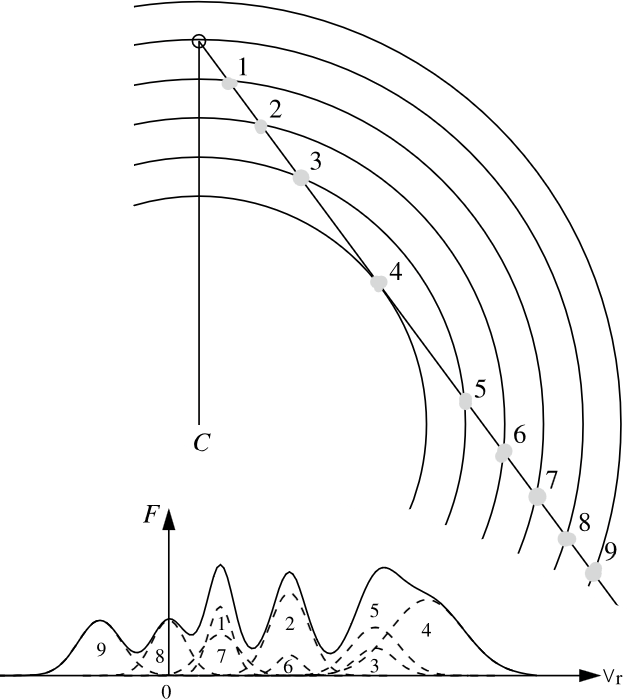
\includegraphics[width=0.95\textwidth]{assets/clouds.png}
    \vspace{-0.3 em}
    \captionof{figure}{Clouds at different distances produce emission lines with different shifts \cite{karttunen}.}
\end{minipage}

\begin{observationblock}[Uncertainties in kinematic mapping]
    Interpreting spiral structure from 21\,cm data is not straightforward. Kinematic distances depend on the rotation curve $V(R)$, but that curve is also estimated from radial velocity measurements, so the method is partly circular. In the inner Galaxy ($|l| < 90^\circ$), the same radial velocity can come from two different distances, creating the \textbf{near/far distance ambiguity}. Also, gas motions that are not perfectly circular, making the distance estimate less accurate.
\end{observationblock}

\subsubsection{Oort's Limit}

By analyzing the vertical kinematics of stars oscillating perpendicularly to the Galactic plane, we can estimate the total local mass density required to gravitationally bind them. This dynamical estimate is known as the \textbf{Oort limit} (1932). Originally, Oort calculated a \textbf{dynamical mass density} that was roughly twice the density accounted for purely by the \textbf{luminosity of observed stars}.

Historically, this discrepancy between the dynamically inferred mass and the visible stellar mass provided one of the earliest hints of "missing mass" in the Universe. However, Oort's early calculations could not fully account for the Interstellar Medium (ISM), comprising cold gas and dust clouds, nor the abundance of very faint red and brown dwarfs.

Modern observations (e.g., from the \textit{Gaia} mission) have largely resolved this local tension. When the mass of the ISM and faint stellar populations are added to the visible luminous mass, the total local density closely matches the dynamical Oort limit. 

This local agreement is profound: it demonstrates that \textbf{dark matter does not flatten into the Galactic disk}. Instead, as large-scale rotation curves reveal, the missing mass must reside in a vast, diffuse spherical halo encompassing the entire Galaxy.

\subsubsection{The Galactic Rotation Curve and Dark Matter}

By observing the 21\,cm line at different Galactic longitudes and applying the \textbf{tangent-point method}, one can determine the angular velocity $\omega(R)$ and the corresponding circular velocity $V(R) = \omega(R)\,R$ for a range of Galactocentric distances. The result is the \textbf{rotation curve} of the Milky Way:

\medskip


\begin{minipage}{0.69\textwidth}
    \centering
    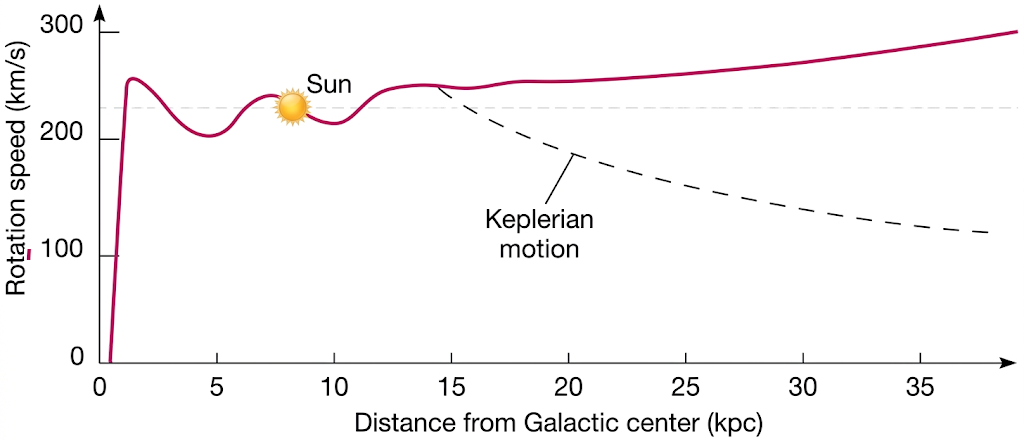
\includegraphics[width=0.97\textwidth]{assets/rot-curve.png}
\end{minipage}%
\hfill
\begin{minipage}{0.26\textwidth}
\captionof{figure}{Rotation curve of the Milky Way from hydrogen clouds. The dashed line shows the Keplerian decline for mass within 20\,kpc \cite{cosmology}.}
\end{minipage}

\medskip

Within the luminous disk ($R \lesssim 10\,\mathrm{kpc}$), the curve rises and then flattens. Beyond the end of the \textbf{luminosity disk}, however, one would naively expect the velocity to follow a \textbf{Keplerian decline}:


$$
V(R) = \sqrt{\frac{GM(<R)}{R}} \quad \xrightarrow{M = \text{const}} \quad V \propto R^{-1/2}
$$
Instead, observations show that $V(R)$ \textit{remains approximately constant} well beyond the luminous extent of the disk. Since $V = \text{const}$ implies $M(<R) \propto R$, the enclosed mass keeps growing with radius even where there are no visible stars or gas. This is direct evidence for the existence of \textbf{dark matter} in an extended halo surrounding the Galaxy.
The total estimated mass of the Milky Way (including the dark matter halo) is:
$$
M_\mathrm{MW} \sim 10^{12}\,M_\odot
$$
which is roughly an order of magnitude larger than the mass in visible stars and gas alone.

\subsection{Applications and Worked Examples}

Oort's constants, kinematic distance determination, and the rotation curve have a wide range of practical applications. Here we present a few key examples.

\subsubsection{1. Distribution of Stars in the Universe.}

Let us suppose that stars are \textbf{uniformly distributed} in space and all have the same absolute magnitude $M$ (a simplifying assumption). The number of stars $N$ brighter than apparent magnitude $m$ is proportional to the volume of space surveyed out to the corresponding distance $s$:
$$
m - M = 5\log s - 5 \quad \Longrightarrow \quad s = 10^{0.2(m-M+5)}
$$
Since $N \propto s^3 \propto 10^{0.6m}$ (the $M$ and constant terms absorb into the proportionality), we obtain:
$$
\log N(m) \propto 0.6\,m
$$
In other words, for a uniform, complete survey, the log of the star counts should increase linearly with apparent magnitude with slope $0.6$.

Any deviation from this slope carries physical information. In particular, the \textbf{Wolf diagram} plots $\log N$ versus $m$ along a specific line of sight: a sudden change in slope (a flattening) signals the presence of an interstellar dust cloud that absorbs light, reducing the number of observable sources beyond a certain distance. From the magnitude at which the break occurs, one can estimate the distance of the cloud.

\begin{figure}[H]
    \centering
    \begin{minipage}{0.48\textwidth}
        \centering
        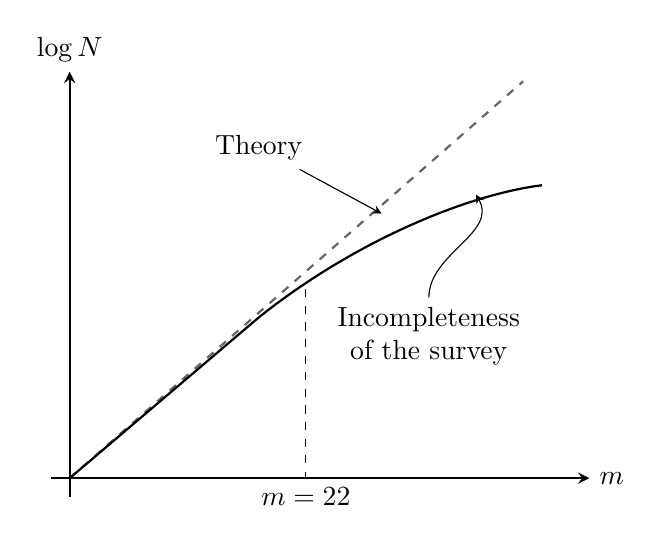
\begin{tikzpicture}[scale=1.2, >=stealth]
            % Axes (slightly wider than tall for the desired proportions)
            \draw[->, thick] (-0.2, 0) -- (5.5, 0) node[right] {$m$};
            \draw[->, thick] (0, -0.2) -- (0, 4.3) node[above] {$\log N$};

            % Theoretical line (uniform distribution)
            \draw[dashed, thick, gray!80!black] (0, 0) -- (4.8, 4.2);

            % Observed curve (survey incompleteness)
            \draw[thick, black] (0, 0) -- (2.0, 1.7) 
                .. controls (3.0, 2.5) and (4.2, 3) .. (5.0, 3.1);

            % Demarcation line at m=22
            \draw[dashed, thin] (2.5, 2) -- (2.5, 0);
            \node[below] at (2.5, 0) {$m=22$};

            % Labels and arrows
            \node (theory_label) at (2.0, 3.5) {Theory};
            \draw[->] (theory_label) -- (3.3, 2.8);

            \node[align=center] (incomp_label) at (3.8, 1.5) {Incompleteness \\ of the survey};
            \draw[->, out=90, in=-60] (incomp_label) to (4.3, 3.0);
        \end{tikzpicture}
        \captionof{figure}{Expected $\log N(m)$ vs.\ $m$ for a uniform star distribution (straight line with slope 0.6), compared to observations.}
    \end{minipage}
    \hfill
    \begin{minipage}{0.49\textwidth}
        \centering
        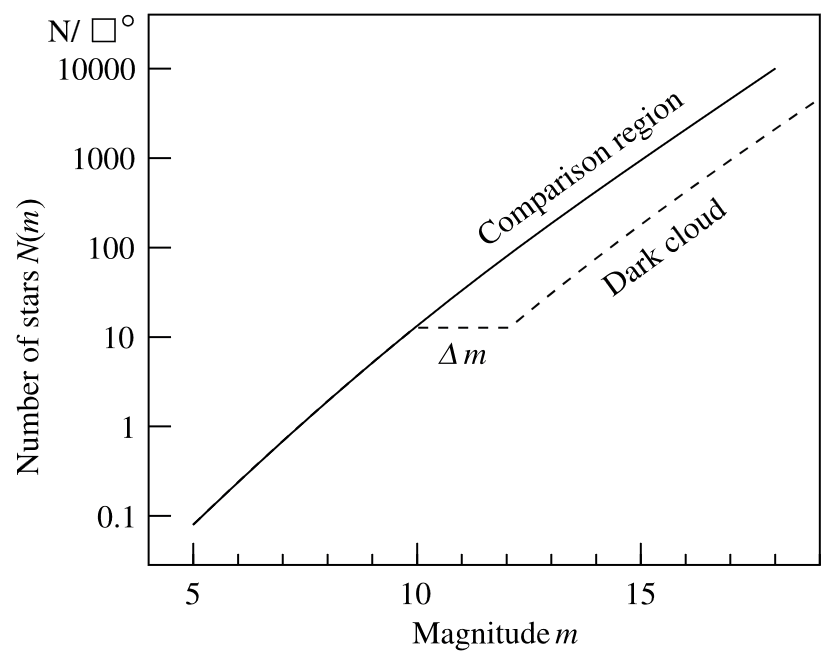
\includegraphics[width=\textwidth]{assets/wolf-diagram.png}
        \captionof{figure}{Wolf diagram: $\log N$ vs.\ $m$ along a line of sight. A flattening of the slope indicates the presence of an absorbing ISM cloud.}
    \end{minipage}
\end{figure}

\subsubsection{2. Cepheid Distance Determination}

Consider a Cepheid with a radial velocity of $80$ km s$^{-1}$, located at a galactic longitude of $145^\circ$. Its period is $3.16$ days, and its apparent visual magnitude is $12.3$. How far away is this star? There are two main approaches to determine its distance:

\begin{itemize}
    \item \textbf{Kinematic Distance (using Oort's Formula):}

    For stars in the solar neighborhood ($r \ll R_0$), their observed radial velocity $v_r$ at a given Galactic longitude $l$ relates to their distance $r$ from the Sun according to Oort's formula:
    $$
    v_r \approx A\,r\,\sin 2l
    \qquad \Rightarrow \qquad
    r = \frac{v_r}{A\sin 2l}
    $$
    Knowing both the radial velocity and the Galactic longitude, we can estimate the distance:
    $$
    r = \frac{80}{14.8 \cdot \sin 90^\circ} \approx 5~\mathrm{kpc}
    $$

    \item \textbf{Photometric Distance (using the Period-Luminosity Relation):}

    The period-luminosity relation tells us that the Cepheid's absolute magnitude is roughly $M \approx -3$. The distance can then be determined from the distance modulus:
    $$
    r = 10^{0.2(m - M + 5)}
    $$
    Plugging in the given numbers,
    $$
    r = 10^{0.2(12.3 + 3 + 5)} = 10^{0.2 \times 20.3} \approx 10~\mathrm{kpc}
    $$
\end{itemize}

The fact that these kinematic and photometric distances differ by nearly a factor of two highlights some important caveats:
\begin{enumerate}
    \item Oort's approximation is valid only near the Sun ($r \ll R_0 \approx 8\,\mathrm{kpc}$), and does not include non-circular or streaming motions.
    \item The photometric distance, based only on the Cepheid's intrinsic brightness, ignores extinction.
    \item Additional velocity components due to random motion can affect the kinematic calculation.
\end{enumerate}